\documentclass[9pt]{article}
\usepackage[left=.5in, right=.5in, top=1in]{geometry}

\usepackage{graphicx}					
\usepackage{amssymb}
\usepackage{float}
\usepackage{url}
\usepackage{graphicx}					
\usepackage{import}
\usepackage{dcolumn}
\usepackage{amssymb}
\usepackage{adjustbox}

\title{Foreign Aid and Soft Power}
\author{.}

% ------------------------------------------------------------------------------------
\begin{document}
\maketitle
\tableofcontents

\setlength{\tabcolsep}{5pt}


% ------------------------------------------------------------------------------------
\newpage
\section{Body of Paper}

\begin{figure}[H]
\centering
\includegraphics[width=1\textwidth]{figures/figure_01.png}
\caption{FIGURE 1: Effects of Chinese and US aid on perceptions of China and the US}
\end{figure}

\begin{figure}[H]
\centering
\includegraphics[width=1\textwidth]{figures/figure_02.png}
\caption{FIGURE 2: Effects of Chinese and US aid on liberal democratic values}
\end{figure}

\begin{figure}[H]
\centering
\includegraphics[width=1\textwidth]{figures/figure_03.png}
\caption{FIGURE 3: Effects of Chinese and US aid on perceptions of former colonial powers}
\end{figure}

\begin{figure}[H]
\centering
\includegraphics[width=1\textwidth]{figures/figure_04.png}
\caption{FIGURE 4: Effects of Chinese aid on factors contributing to positive image of China}
\end{figure}

\begin{figure}[H]
\centering
\includegraphics[width=1\textwidth]{figures/figure_05.png}
\caption{FIGURE 5: Effects of Chinese aid on factors contributing to negative image of China}
\end{figure}


% ------------------------------------------------------------------------------------
\appendix
\section{Appendix 1: Coding Rules and Descriptive Statistics}

\begin{figure}[H]
\centering
%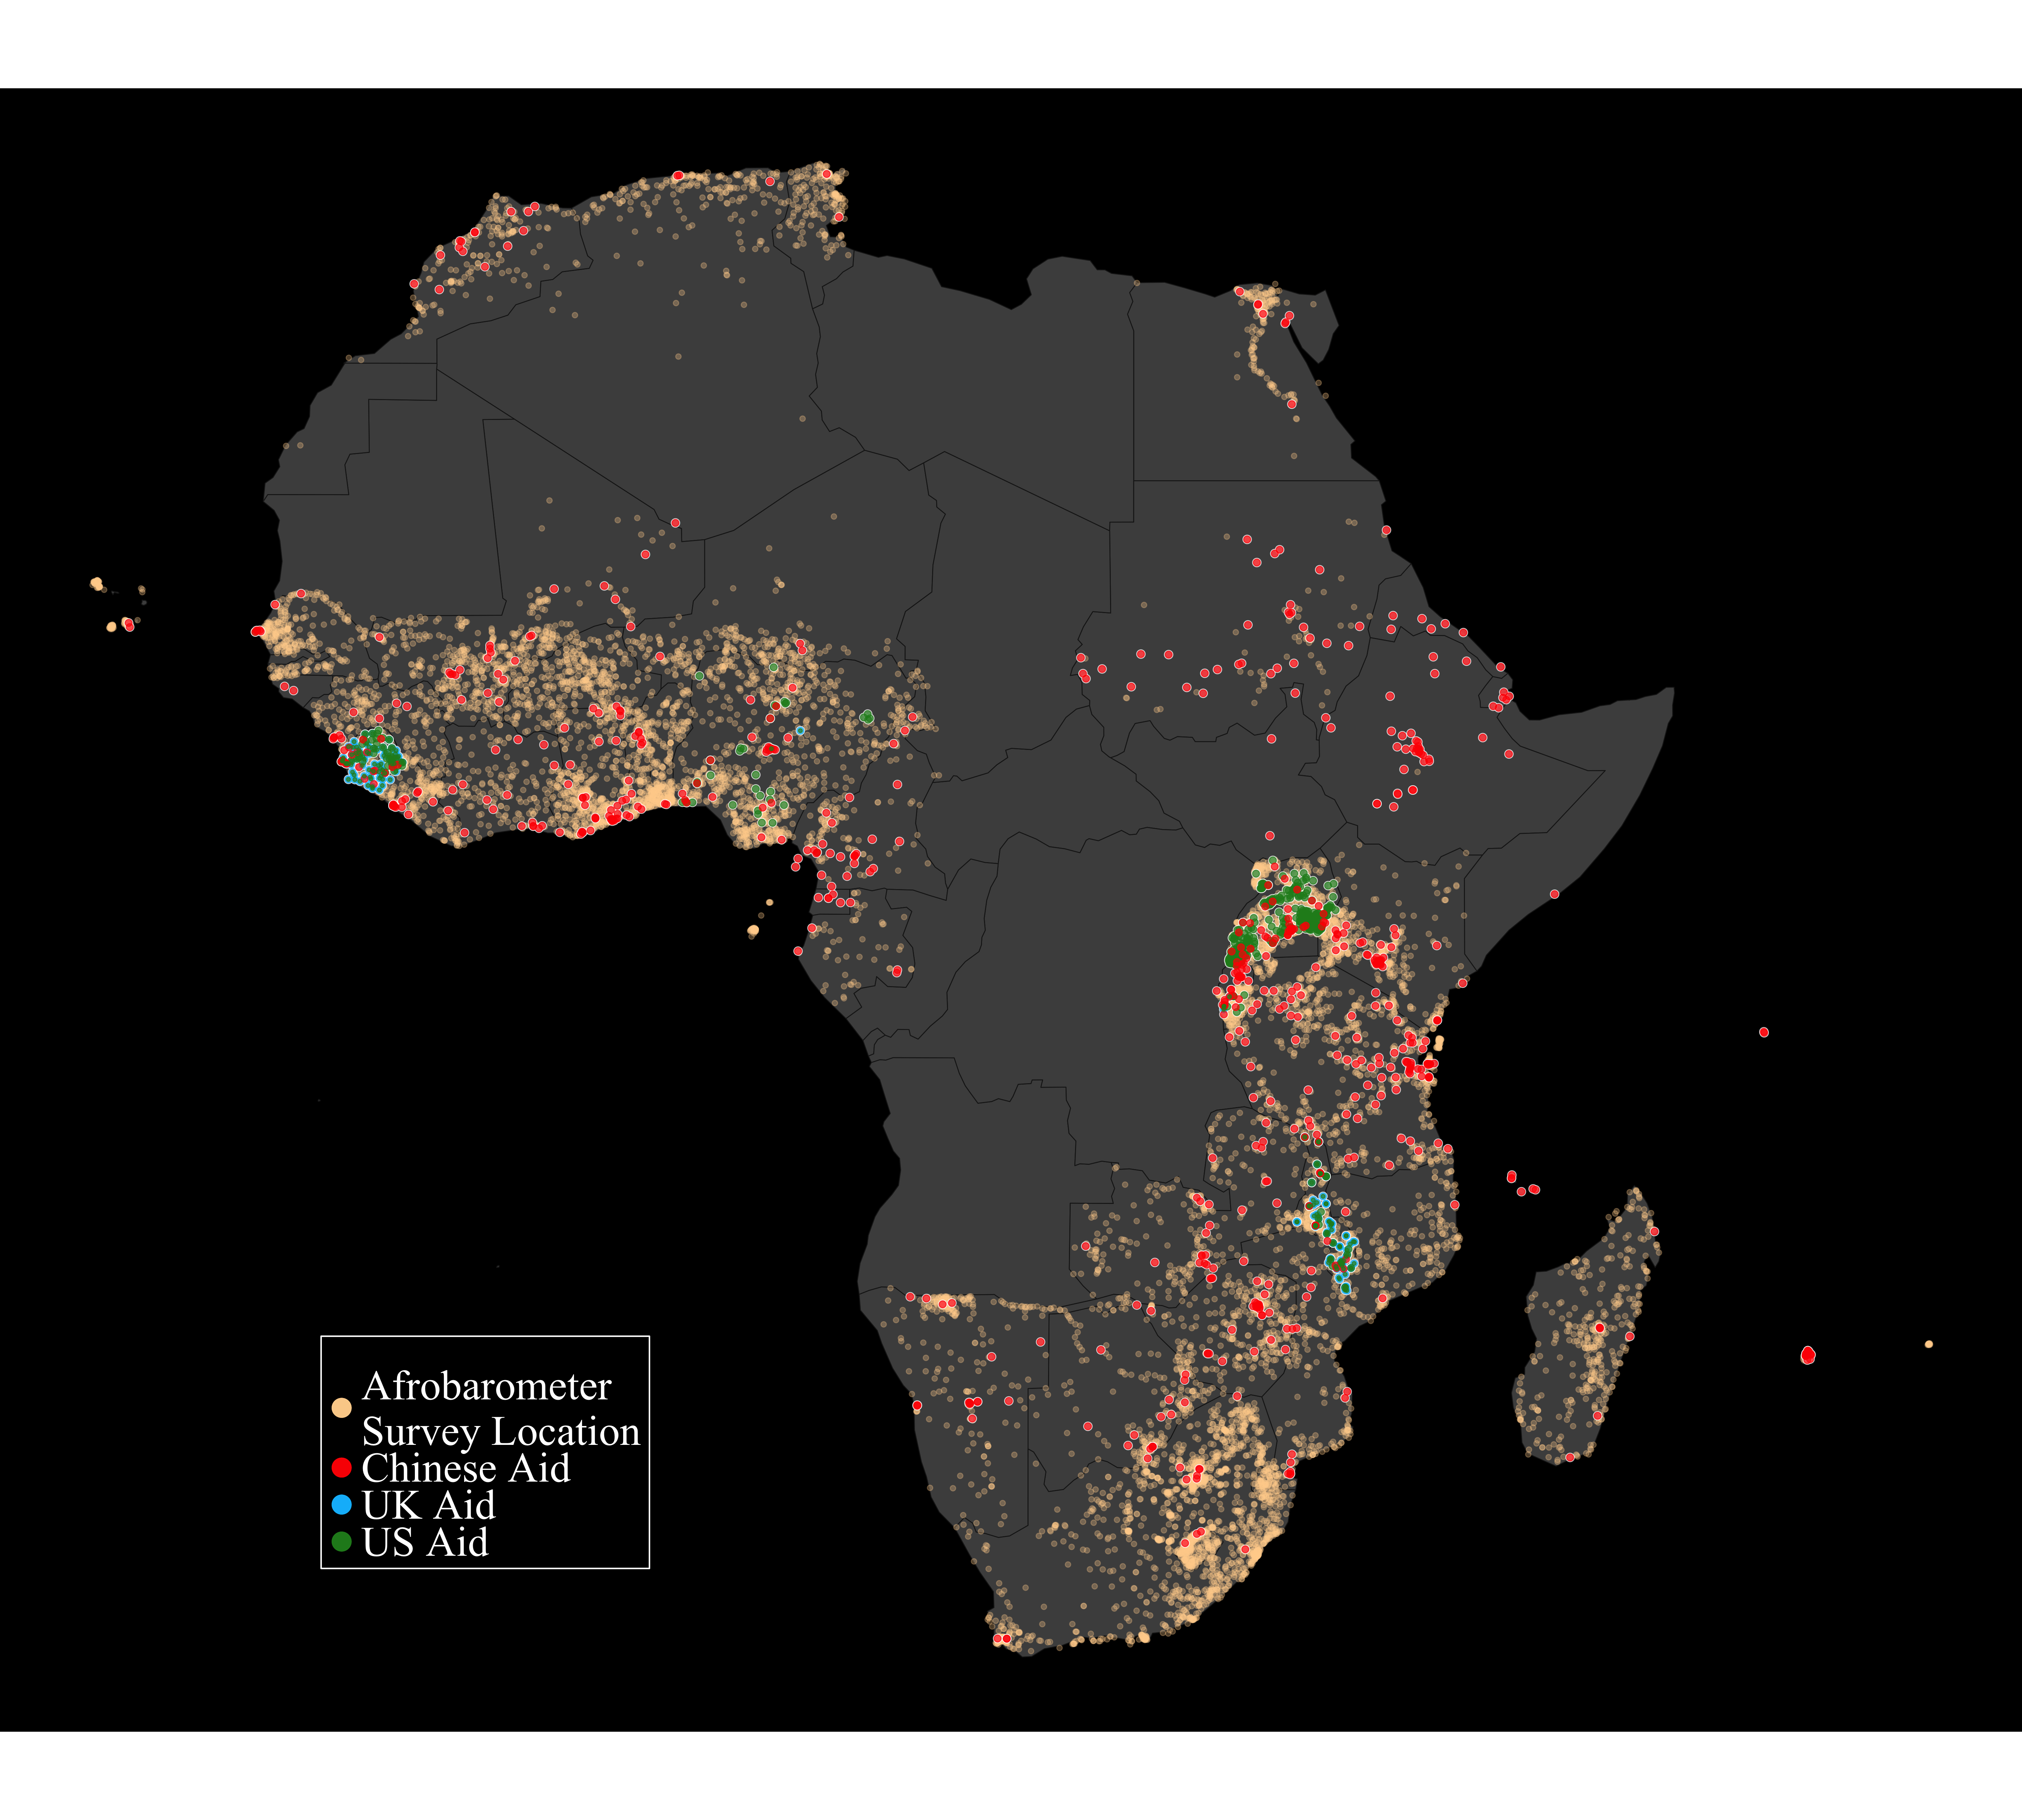
\includegraphics[width=1\textwidth]{figures/figure_a1.png}
\caption{FIGURE A1: Map of Afrobarometer respondents and Chinese, US, and UK aid projects}
\end{figure}

\begin{figure}[H]
\centering
\includegraphics[width=0.3\textwidth]{figures/figure_a2.png}
\caption{FIGURE A2: Distribution of Chinese projects by country in full sample}
\end{figure}

\begin{figure}[H]
\centering
\includegraphics[width=0.7\textwidth]{figures/figure_a3.png}
\caption{FIGURE A3: Distribution of Chinese, US, and UK projects by country in restricted sample}
\end{figure}

\setlength{\tabcolsep}{5pt}
\begin{table}[H]
\caption{TABLE A1: Descriptive statistics on independent variables}
\label{reg}
\centering
\import{tables/}{table_a1.tex}
\end{table}

\setlength{\tabcolsep}{5pt}
\begin{table}[H]
\caption{TABLE A2: Descriptive statistics on dependent variables}
\label{reg}
\centering
\import{tables/}{table_a2.tex}
\end{table}

\setlength{\tabcolsep}{5pt}
\begin{table}[H]
\caption{TABLE A3: Descriptive statistics on control variables}
\label{reg}
\centering
\import{tables/}{table_a3.tex}
\end{table}

\setlength{\tabcolsep}{5pt}
\begin{table}[H]
\caption{TABLE A4: Comparison of Chinese projects in full sample and our sample by sector}
\label{reg}
\centering
\import{tables/}{table_a4.tex}
\end{table}

\setlength{\tabcolsep}{5pt}
\begin{table}[H]
\caption{TABLE A5: Comparison of US projects in full sample and our sample by sector}
\label{reg}
\centering
\import{tables/}{table_a5.tex}
\end{table}

\setlength{\tabcolsep}{5pt}
\begin{table}[H]
\caption{TABLE A6: Comparison of completed and planned Chinese projects by sector}
\label{reg}
\centering
\import{tables/}{table_a6.tex}
\end{table}

\setlength{\tabcolsep}{5pt}
\begin{table}[H]
\caption{TABLE A7: Comparison of completed and planned US projects by sector}
\label{reg}
\centering
\import{tables/}{table_a7.tex}
\end{table}

% ------------------------------------------------------------------------------------
\newpage
\section{Appendix 2: Robustness Checks}

% ------------------------------------------------------------------------------------
\newpage
\section{Appendix 3: Extensions}


\end{document}  
















